\documentclass[11pt,a4paper]{article}
\usepackage[utf8]{inputenc}
\usepackage[spanish]{babel}	%Idioma
\usepackage{amsmath}
\usepackage{amsfonts}
\usepackage{amssymb}
\usepackage{graphicx} 	%Añadir imágenes
\usepackage{geometry}	%Ajustar márgenes
\usepackage[export]{adjustbox}[2011/08/13]
\usepackage{float}
\restylefloat{table}
\usepackage[hidelinks]{hyperref}
\usepackage{titling}
\graphicspath{{/home/nazaret/Escritorio/LaTEX}}
%\usepackage{minted}
\usepackage{multirow}
\usepackage{caption}
\usepackage{multicol}
\usepackage[shortlabels]{enumitem}
\usepackage{array}
\selectlanguage{spanish}

%Opciones de encabezado y pie de página:
\usepackage{fancyhdr}
\pagestyle{fancy}
\lhead{Nazaret Román Guerrero}
\rhead{la asignatura}
\lfoot{Grado en Ingeniería Informática}
\cfoot{}
\rfoot{\thepage}
\renewcommand{\headrulewidth}{0.4pt}
\renewcommand{\footrulewidth}{0.4pt}

%Opciones de fuente:
\usepackage[utf8]{inputenc}
\usepackage[default]{sourcesanspro}
\usepackage{sourcecodepro}
\usepackage[T1]{fontenc}

\setlength{\parindent}{15pt}
\setlength{\headheight}{15pt}
\setlength{\voffset}{10mm}

% Custom colors
\usepackage{color}
\definecolor{deepblue}{rgb}{0,0,0.5}
\definecolor{deepred}{rgb}{0.6,0,0}
\definecolor{deepgreen}{rgb}{0,0.5,0}

\usepackage{listings}

\begin{document}
\begin{titlepage}

\begin{minipage}{\textwidth}

\centering
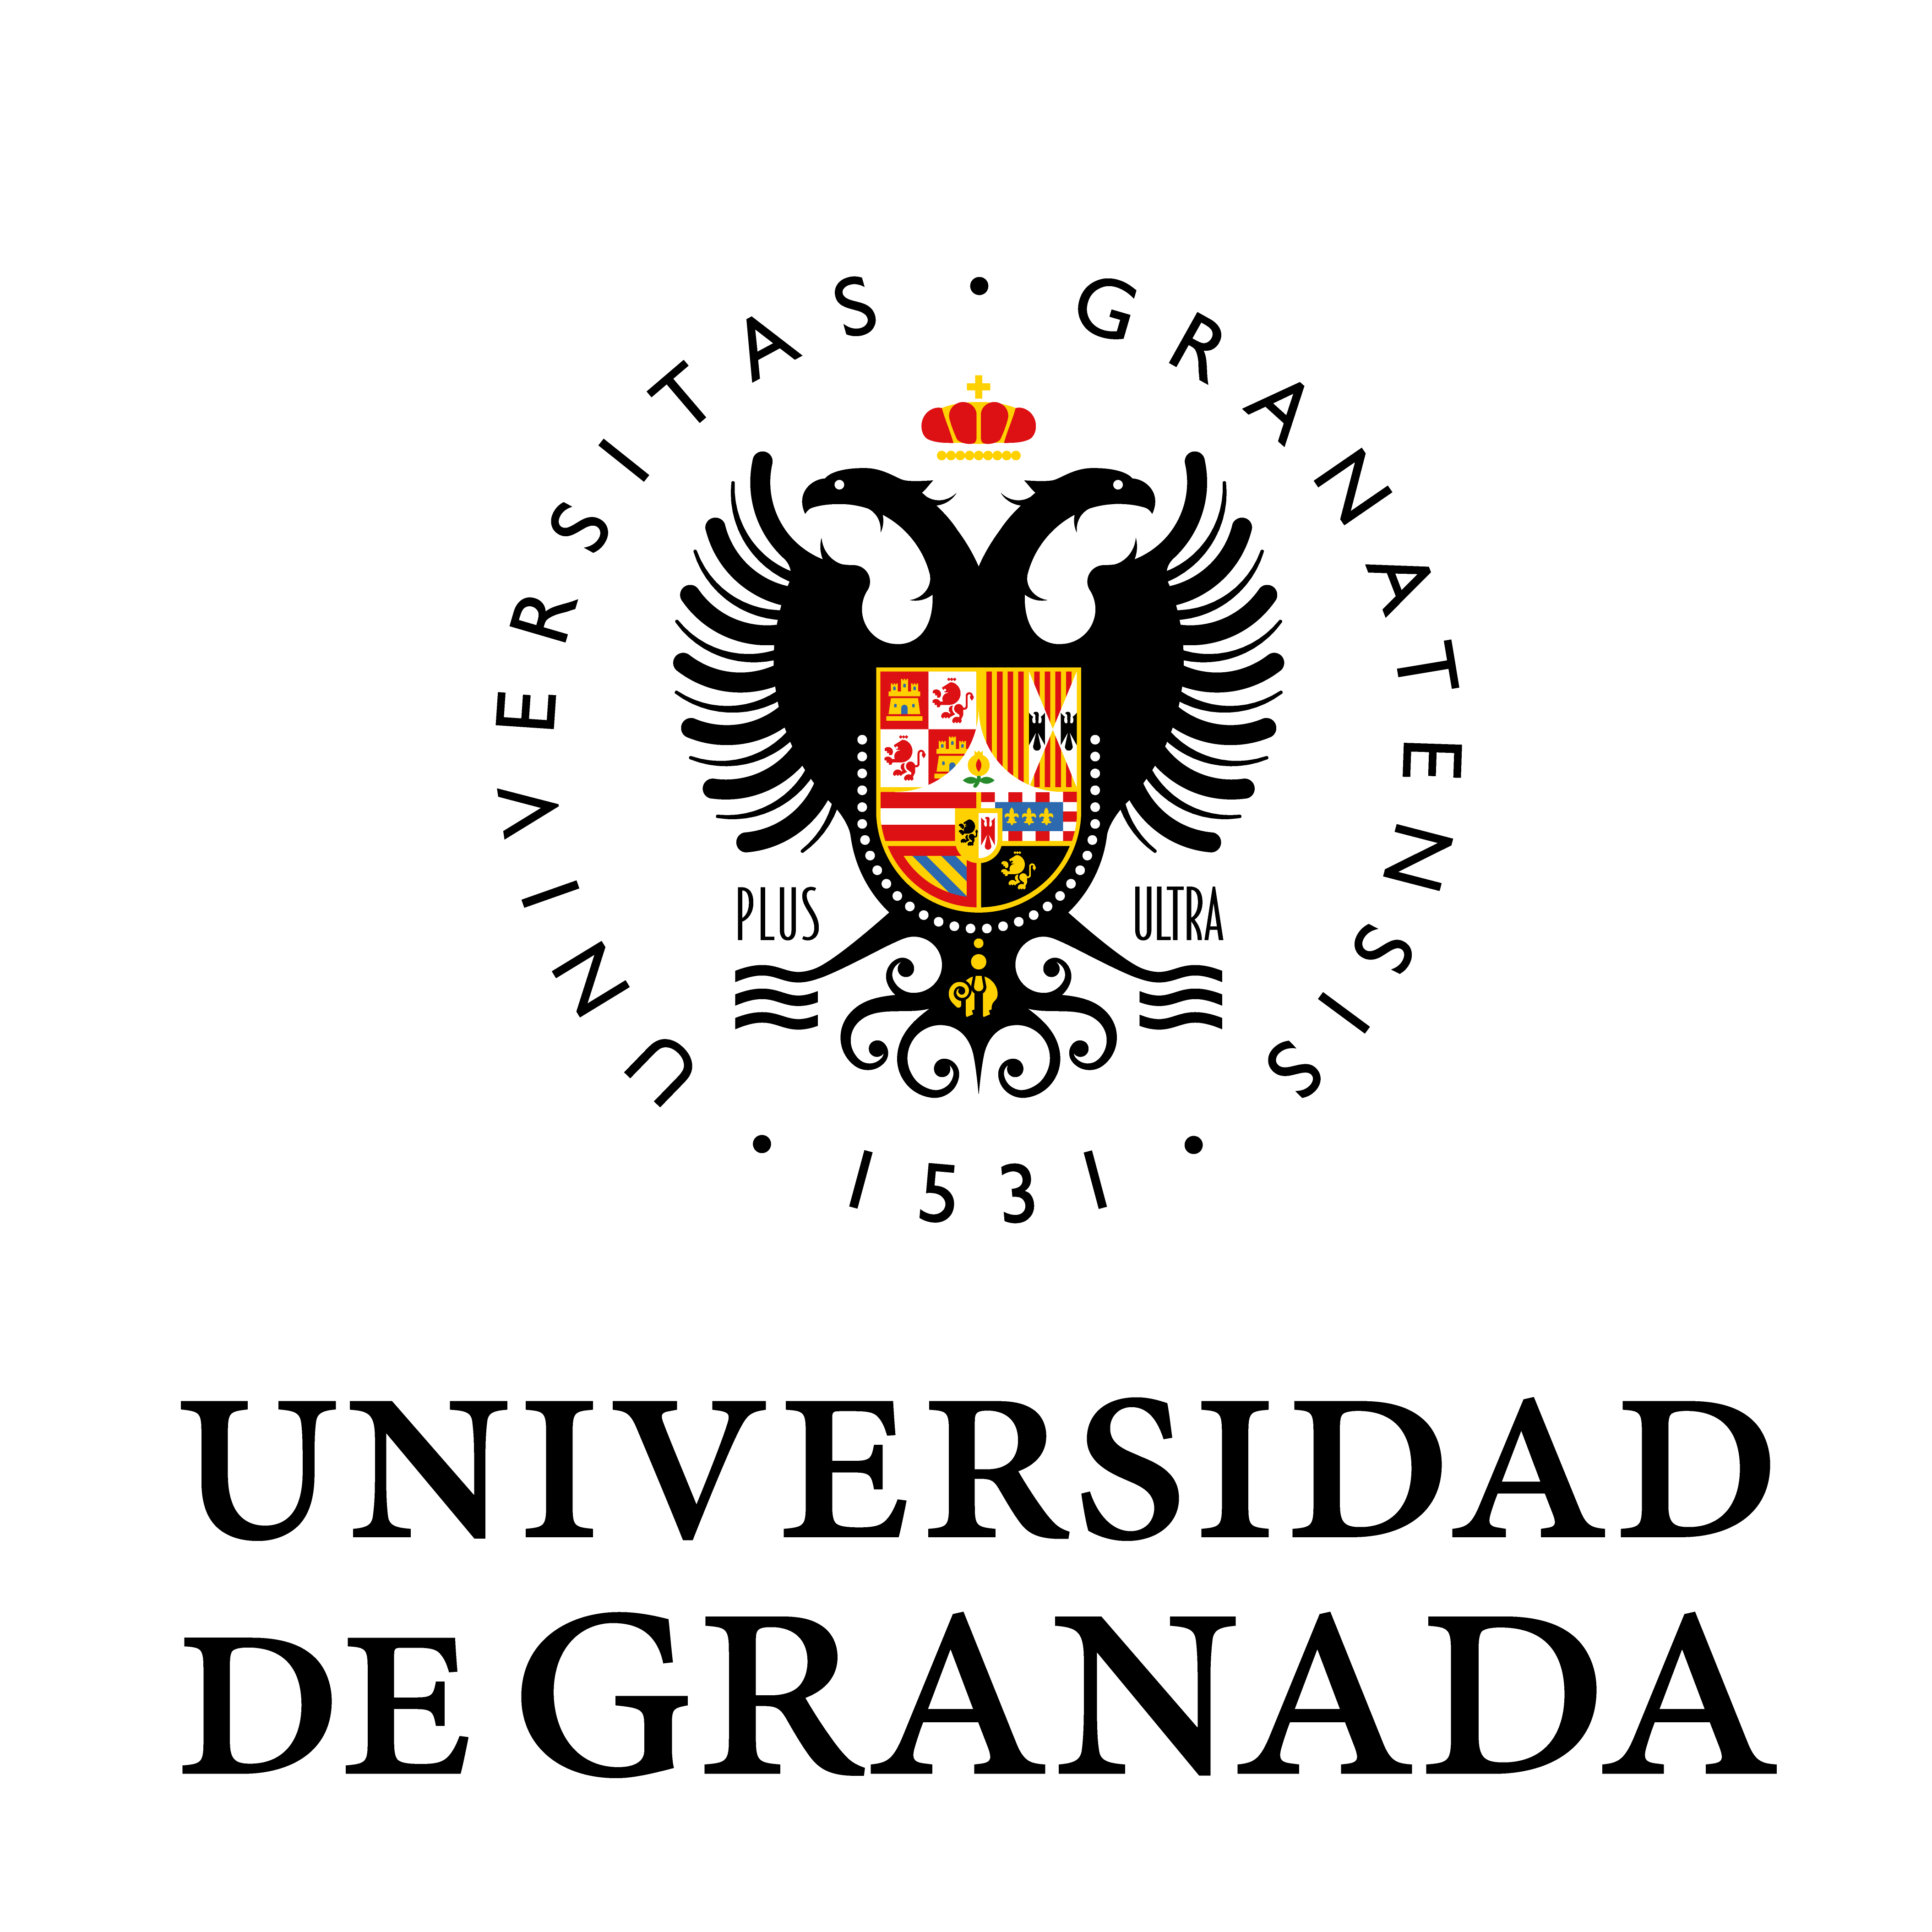
\includegraphics[width=0.5\textwidth]{img/logo.png}\\

\textsc{\Large asignatura\\[0.2cm]}
\textsc{GRADO EN INGENIERÍA INFORMÁTICA}\\[1cm]

{\Huge\bfseries practica\\}
\noindent\rule[-1ex]{\textwidth}{3pt}\\[3.5ex]
{\large\bfseries subpractica}
\end{minipage}

\vspace{1.5cm}
\begin{minipage}{\textwidth}
\centering

\textbf{Autora}\\ {Nazaret Román Guerrero}\\[2.5ex]

\includegraphics[width=0.3\textwidth]{img/etsiit.jpeg}\\[0.1cm]
\vspace{1cm}
\textsc{Escuela Técnica Superior de Ingenierías Informática y de Telecomunicación}\\
\vspace{1cm}
\textsc{Curso 2018-2019}
\end{minipage}
\end{titlepage}

\pagenumbering{gobble}
\pagenumbering{arabic}
\tableofcontents
\thispagestyle{empty}

\newpage

\section{Cómo funciona un corazón}

El corazón actúa como  una bomba que reparte sangre por el organismo. Para que ese ocurra, el corazón emite latidos gracias a impulsos nerviosos que funcionan como señales eléctricas generadas por el cerebro, que provocan la contracción y relajación de las cavidades del órgano, las aurículas y los ventrículos.\\

Los impulsos eléctricos contraen el corazón que impulsa la sangre por las arterias, el medio por el cual llegan al resto del cuerpo. De vuelta al corazón, las venas llevan la sangre al órgano para poder purificarla y añadirle oxígeno limpio.

\section{Pulsos eléctricos del corazón}

Cuando un corazón no es capaz de latir por sí solo, puede ser causar dos eventos: que el corazón se pare totalmente, por lo que hay que reactivarlo mediante una descarga eléctrica de magnitudes considerables, entre 1500 y 2200 voltios, para reanimarlo. A esto se le llama ataque cardíaco.\\

El segundo evento puede ser la ralentización del ritmo cardíaco sin que se llegue a parar. Esto se denomina bradicardia, y para evitar males mayores se instala un pequeño dispositivo en el corazón que provoca la contracción del corazón por impulsos eléctricos. Este dispositivo se denomina marcapasos.

\section{Señales eléctricas de bombeo}

El corazón genera ondas causadas por los impulsos eléctricos de forma que la sangre se mueve por el corazón para dirigirse a las distintas partes del cuerpo.\\

Un marcapasos actua igual: genera los impulsos eléctricos con precisión para que la contracción del corazón sea suficiente para enviar la sangre pero no muy alta par no isquemiar los músculos del órgano, es decir, darles un impulso tan fuerte que paralices a las células que lo forma.\\

El marcapasos está formado por una batería de litio de larga duración, un generador de impulsos, un captador o detector de la actividad cardiaca y el electrodo que lo conecta con el corazón.\\

\section{Latidos del corazón. Frecuencia y amplitud}

El corazón pasa por diferentes fases que se observan en el latido:

\begin{enumerate}
	\item Onda P. Corresponde a la contracción de las aurículas. La sangre pasa de las aurículas a los ventrículos.
	\item Complejo QRS. Corresponde a la contracción de los ventrículos. La sangre sale del corazón a los pulmones o al resto del cuerpo.
	\item Onda T. Corresponde a la repolarización de los ventrículos, es decir, se vuelven a llenar de la sangre que viene del resto del cuerpo.
\end{enumerate}

Los segmentos e intervalos PR, ST y QT son los determinantes de problemas del corazón: arritmias, bloqueos, infartos, isquemias de miocardio...

\section{Generador de impulsos}

El detector de actividad cardíaca registra los latidos del corazón mediante el electrodo conectado. Cuando se detecta que el ritmo cardíaco es peor del que debería, los circuitos del detector comunican la información al generador de impulsos.\\

El generador de impulsos recibe la frecuencia cardíaca y se pone en funcionamiento según dicha frecuencia a la que está funcionando. El generador lanza impulsos con la frecuencia y amplitud necesaria para poner al corazón en funcionamiento normal y que siga bombeando sangre.\\

El umbral a partir del que se detecta que el corazón no está funcionando correctamente es muy importante, pues es el que determinará si se debe avisar al generador de impulsos de qué generen ondas o no. Si el umbral es demasiado bajo, el marcapasos sobreefectuará los latidos y provocará una taquicardia de mayor o menor nivel que puede acabar con la vida del paciente; por otro lado, si el umbra es demasiado alto, el marcapasos no reaccionará cuando debe y causará una bradicardia al paciente (será causada por su propio corazón al ser incapaz de latir por sí solo) que puede acabar también con la vida del paciente.\\

Para la captura del pulso requiere de dos parámetros:

\begin{itemize}
	\item Amplitud. Refleja la altura del pulso, es decir, la fuerza del latido.
	\item Período. Refleja la duración del ciclo completo de un solo latido del corazón. Es gracias a este factor que se pueden detectar problemas cardíacos como bloqueos o arrítmias.
\end{itemize}

\end{document}